%\documentclass{report}
\documentclass{article}

\usepackage[utf8]{inputenc}
\usepackage{txfonts}
\usepackage{rotating}
\usepackage{amssymb}
\usepackage{natbib}
\usepackage{varioref}
%

\begin{document}



%\vskip1cm
%
%  These Macros are taken from the AAS TeX macro package version 4.0.
%  Include this file in your LaTeX source only if you are not using
%  the AAS TeX macro package and need to resolve the macro definitions
%  in the BibTeX entries returned by the ADS abstract service.
%
%  For more information on the AASTeX macro package, please see the URL
%	http://www.ferberts.com/AAS/aastex.html
%  For more information about ADS abstract server, please see the URL
%	http://adswww.harvard.edu/ads_abstracts.html
%

% Abbreviations for journals.  The object here is to provide authors
% with convenient shorthands for the most "popular" (often-cited)
% journals; the author can use these markup tags without being concerned
% about the exact form of the journal abbreviation, or its formatting.
% It is up to the keeper of the macros to make sure the macros expand
% to the proper text.  If macro package writers agree to all use the
% same TeX command name, authors only have to remember one thing, and
% the style file will take care of editorial preferences.  This also
% applies when a single journal decides to revamp its abbreviating
% scheme, as happened with the ApJ (Abt 1991).

\def\aj{\rm{Astronomical Journal}}                   % Astronomical Journal
\def\araa{\rm{ARA\&A}}             % Annual Review of Astron and Astrophys
\def\apj{\rm{Astrophysical Journal}}                 % Astrophysical Journal
\def\apjl{\rm{Astrophysical Journal, Letters}}                % Astrophysical Journal, Letters
\def\apjs{\rm{Astrophysical Journal, Supplement}}               % Astrophysical Journal, Supplement
\def\ao{\rm{Appl.~Opt.}}           % Applied Optics
\def\apss{\rm{Ap\&SS}}             % Astrophysics and Space Science
\def\aap{\rm{Astronomy and Astrophysics}}                % Astronomy and Astrophysics
\def\aapr{\rm{Astronomy and Astrophysics Reviews}}          % Astronomy and Astrophysics Reviews
\def\aaps{\rm{Astronomy and Astrophysics, Supplement}}              % Astronomy and Astrophysics, Supplement
\def\azh{\rm{AZh}}                 % Astronomicheskii Zhurnal
\def\baas{\rm{BAAS}}               % Bulletin of the AAS
\def\jrasc{\rm{JRASC}}             % Journal of the RAS of Canada
\def\memras{\rm{MmRAS}}            % Memoirs of the RAS
\def\mnras{\rm{Monthly Notices of the RAS}}             % Monthly Notices of the RAS
\def\pra{\rm{Phys.~Rev.~A}}        % Physical Review A: General Physics
\def\prb{\rm{Phys.~Rev.~B}}        % Physical Review B: Solid State
\def\prc{\rm{Phys.~Rev.~C}}        % Physical Review C
\def\prd{\rm{Phys.~Rev.~D}}        % Physical Review D
\def\pre{\rm{Phys.~Rev.~E}}        % Physical Review E
\def\prl{\rm{Phys.~Rev.~Lett.}}    % Physical Review Letters
\def\pasp{\rm{Publications of the ASP}}               % Publications of the ASP
\def\pasj{\rm{PASJ}}               % Publications of the ASJ
\def\qjras{\rm{QJRAS}}             % Quarterly Journal of the RAS
\def\skytel{\rm{S\&T}}             % Sky and Telescope
\def\solphys{\rm{Sol.~Phys.}}      % Solar Physics
\def\sovast{\rm{Soviet~Ast.}}      % Soviet Astronomy
\def\ssr{\rm{Space~Sci.~Rev.}}     % Space Science Reviews
\def\rmxaa{\rm{Rev.Mex. de Astronomia y Astrofisica}}    
\def\zap{\rm{ZAp}}                 % Zeitschrift fuer Astrophysik
\def\nat{\rm{Nature}}              % Nature
\def\iaucirc{\rm{IAU~Circ.}}       % IAU Cirulars
\def\aplett{\rm{Astrophys.~Lett.}} % Astrophysics Letters
\def\apspr{\rm{Astrophys.~Space~Phys.~Res.}}
                % Astrophysics Space Physics Research
\def\bain{\rm{Bull.~Astron.~Inst.~Netherlands}} 
                % Bulletin Astronomical Institute of the Netherlands
\def\fcp{\rm{Fund.~Cosmic~Phys.}}  % Fundamental Cosmic Physics
\def\gca{\rm{Geochim.~Cosmochim.~Acta}}   % Geochimica Cosmochimica Acta
\def\grl{\rm{Geophys.~Res.~Lett.}} % Geophysics Research Letters
\def\jcp{\rm{J.~Chem.~Phys.}}      % Journal of Chemical Physics
\def\jgr{\rm{J.~Geophys.~Res.}}    % Journal of Geophysics Research
\def\jqsrt{\rm{J.~Quant.~Spec.~Radiat.~Transf.}}
                % Journal of Quantitiative Spectroscopy and Radiative Trasfer
\def\memsai{\rm{Mem.~Soc.~Astron.~Italiana}}
                % Mem. Societa Astronomica Italiana
\def\nphysa{\rm{Nucl.~Phys.~A}}   % Nuclear Physics A
\def\physrep{\rm{Phys.~Rep.}}   % Physics Reports
\def\physscr{\rm{Phys.~Scr}}   % Physica Scripta
\def\planss{\rm{Planet.~Space~Sci.}}   % Planetary Space Science
\def\procspie{\rm{Proc.~SPIE}}   % Proceedings of the SPIE

\let\astap=\aap
\let\apjlett=\apjl
\let\apjsupp=\apjs
\let\applopt=\ao



%--------------------------------------------------------
\section{Model description}
\label{cap:description}
%--------------------------------------------------------

We follow the analytic model of a photoevaporated wind described in \citet{1998AJ....116..322H} ``Accelerating divergent photoevaporation flow (applied to proplyds)''.
 
The simplest assumpion is that there is a static spherical distribution of gas about the central lowmass star. This gas is being evaporated and ionizing by the radiation coming from $\theta_1 C$


%--------------------------------------------------------
\subsection{Geometry}
\label{cap:geometry}
%--------------------------------------------------------

\begin{itemize}
\item{Radiacion ionizante que incide de manera paralela al proplyd.}
\item{Se asume una geometria cilindrica con simetría en la coordenada $\Phi$}
\item{Frontera de ionizacion semiesferica}
\item{El gas fotoionizado fluye de manera radial de la frontera de ionizacion}
\end{itemize}


El flujo no es isotermico
Las desexcitaciones colisionaes no son despreciables

The Figure1 shows the sketched model, geometry and physical conditions.

Si tomamos un marco de referencia cuyo cero se encuentre en el centro
del proplyd, podemos definir una coordenada espacial adimensional $\rm
R = r / r_0$ donde $\rm r_0$ es la distancia medida observacionalmente
del centro del proplyd a la frontera de ionizacion

\begin{figure}[h]
  \centering
  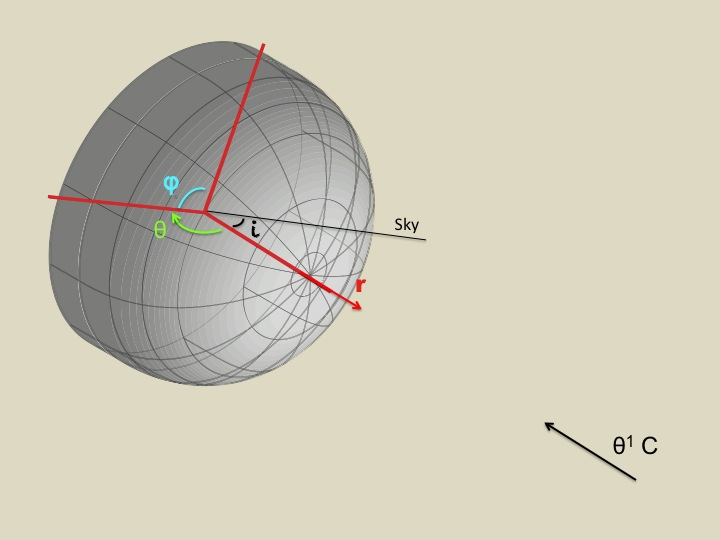
\includegraphics[width=8.5 cm]{./graf_model_3D/geometry_model.jpg}
  \caption{} \label{fig:geometry}
\end{figure}

%-------------------------------------------------------
\subsection{Physical properties}
\label{cap:density}
%-------------------------------------------------------

We divide the proplyd flow into two zones:

\begin{itemize}
  \item{$\rm r > r_0$: An outer, fully ionized, supersonic flow.}
    \item{$\rm r < r_0$: A thin, partially ionized, subsonic ionization front.}
\end{itemize}

This is equivalent to say that the physical properties are diferent in both zones. The boundary between them are exactly the sonic point. The conditions there, and in every point of the proplyd, are fixed by continuity.

In particular, the density that we use is divide into two functions: 

\begin{equation}
  \rm n_e(X) = \left\lbrace
    \begin{array}{l}
      f_1(X) \;\;\;\;\; 1 \ge X \ge 0.98 \\
      f_2(X) \;\;\;\;\;  X \le 0.98 \\
    \end{array}
  \right.
\end{equation}

%-------------------------------------------------------
\subsubsection{The outer zone}
\label{cap:outer}
%-------------------------------------------------------

In the outer zone we assume an isothermal, supersonic, complite ionized flow. From mass conservation, in spherical geometry and In the steady state, radial velocity of the ionized gas, v(r),
satisfies the equation


\begin{equation}
  \rm \rho v r^2 = cte
\end{equation}

%-------------------------------------------------------
\subsubsection{The boundary}
\label{cap:boundary}
%-------------------------------------------------------

The ionization front (I-front) is exactly were the , the Stromgren criterium for a density bounded region:

\begin{equation}
  \rm \phi(H) = \frac{Q(H)}{4\pi D^2} =\alpha_B \int^{\infty}_{r_0}n^2(r) dr
\end{equation}

%-------------------------------------------------------
\subsubsection{The inner zone}
\label{cap:inner}
%-------------------------------------------------------

Partially ionized region: Density is function of sound speed

La ley de densidad usada para el gas completamente ionizado como funcion de la velocidad es

\begin{equation}
  \rm R = U^{(-1/2)} exp (\frac{1}{4} (U^2 -1))
\end{equation}

donde $\rm U(R) = v / c_0$ con $\rm v(R)$ la velocidad del gas y $\rm c_0(R)$ la velocidad del sonido.



Y dentro de la frontera de ionización:

\begin{equation}
  \rm \rho(c_m)
\end{equation}

En cada punto la ecuacion de continuidad, permite calcular la densidad:

\begin{equation}
  \rm \rho (R) v(R) R^2 = \rho (R_{max}) v(R_{max}) R_{max}^2
\end{equation}

%--------------------------------------------------------
\subsection{Calculation}
\label{cap:calculation}
%--------------------------------------------------------

We will construct Cloudy models of a series of individual radial cuts from the center of the proplyd, at different angles $\theta$ from the proplyd axis.

\bibliographystyle{t}

\bibliography{model}

\end{document}
